\chapter{Feature Engineering}
\label{chap:fea}

\todoA{FEATURE SELECTION FOR
KNOWLEDGE DISCOVERY AND
DATA MINING
Huan Liu
Hiroshi Motoda}

\bf Words \rm

 \todoA{- TD*IDF - with given threshholds}

 \todoB{try TD*IDF not with a~given threshold, but rather find te optimal threshold for cuts}

 \todoB{- choose words with highest information gain; as in McCallum Event models}

 \todoA{Fasttext}

\bf Groups of words: \rm

\bf entities extracted from geneea \rm

 \todoB{- filter them based on the~geneea value of importance}

 \todoA{- occurrences - pick only the~most frequent}

\bf simple Bigrams, moregrams\rm

\todoA{- same approach as for unigrams}

\subsection{Later try adding more features (mainly linguistics):}

\todoB{Cosine sim}

\todoA{Spell check}

\todoA{Review length}

\todoB{Stars as non-linguistic feature}

\todoC{Go your imagination wild}

\todoA{What is a feature?? - ref from previous part}

\todoA{do these two paragraphs need citation too?}

\todoB{PCA/SVD reduction}

Features are divided by their values into three categories~---~nominal, ordinal and continuous. Nominal features are discrete and their values do~not convey any relationship. When a~feature is ordinal, it means it is discrete and also convey ordering of the values. Continuous feature is then any real-valued variable.

In this text we will deal with nominal and ordinal only. The simplest way to treat ordinal features is to omit the order. This of course loses information conveyed in this ordering, but will allow us easier feature manipulation.

\section{Commonly Used Features}

\subsection{bag-of-word (BOW)}

\subsubsection{td-idt}

\todoA{source: Using TF-IDF to Determine Word Relevance in Document Queries - downloaded}

\subsubsection{*-gram}




\subsection{Singular Value Decomposition (SVD/PCA)}

\subsection{Word embeddings}

\subsection{hand crafted features}

\subsection{non-textual features --- metadata}



\section{Extraction}

Too many feature -> extraction, selection



\section{Selection}

Machine learning is used in contexts where the true natural and inner logic of~data is~not known. Therefore it is difficult to intuitively select only useful features. Having fewer features which are informative enough leads to three direct benefits.

Trained model is far less complex and as~such easier to~interpret. The~model also generalises better, because the~risk of overfitting is lower. Overfitting happens when the~model recognises irregularities in training data and classifies individual already seen instances, whereas it should approximate the~original model to~be able to~classify unseen instances. Lastly, fewer features result in shorter training time.

Three types of feature selection are generally recognised.



\subsection{Filters}

Filters are popular, because their time complexity is linear in the~number of~features. However, the feature selection may~not be optimal, because neither the~used classificator nor feature correlation is taken into account. When there are highly correlated features, it is unnecessary to choose all of them, because the information conveyed in some may be inferred from others. However, any filter will choose all of them, because filters consider features independently of each other.

Filters work with individual features independently of any supervised classification algorithm. Each feature is used or omitted based on the filter condition. There are number of filters differing in the filter condition.

\subsubsection{PMI}

\subsubsection{MI}

\subsubsection{$\chi^2$}




\subsection{Wrappers}

Unlike filters, wrappers work with subsets of features. Every subset is classified by a classificator used as a black box and then evaluated by some common evaluation metrics. The optimal subset is than chosen. Thanks to this, wrappers are universal and robust.

Furthermore, wrappers can perform a lot better than filters on certain datasets. Such a~case is documented by \citet{GuyEli03} in~\ref{guyeli03-figure3}. The bottom left graph shows the original data and the~top left shows projection onto only one axis. It is clear that one variable cannot be sufficient for separating the clusters. However, if we project the data onto a combination of the two axis, the clusters can be at least partially separated as can be seen in the right part of the figure.
 
 \todoA{citation and vector}

\begin{figure}[ht]\centering
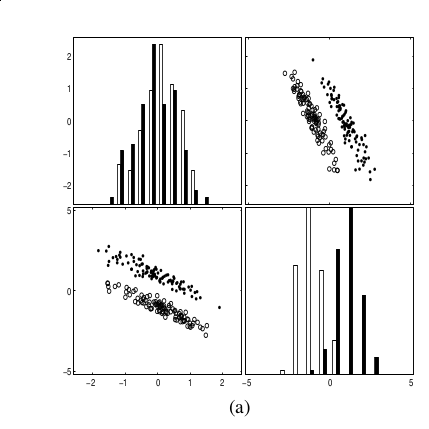
\includegraphics[width=100mm]{../img/guyeli_figure3.png}
\caption{Example of correlated features from the article}
\label{guyeli03-figure3}
\end{figure}

Unfortunately, wrappers tend to be computationally expensive, because every subset must by classified separately. In fact, it has been shown it is NP-hard to find optimal solution. To achieve computational feasibility various approximation methods has been developed. These methods allow us to classify only a fraction of subsets at the cost of losing the guarantee of the optimal solution. We will describe two variants of greedy search.

\todoB{On the approximability of minimizing nonzero variables
or unsatisfied relations in linear systems --- citation of the NP-hard, otherwise delete} 

\subsubsection{Greedy Search --- Forward Selection}

{\it Forward selection} starts with an empty set and in every step adds a feature which brings the highest gain in the evaluation metrics. The feature is selected by adding all of them to the current  subset and evaluating it. The step is repeated until the increase in performance is less than a certain threshold. 

\subsubsection{Greedy Search --- Backward Elimination}

{\it Backward elimination} starts with the set of all features. In one step every feature is removed from the subset and this new subset is than evaluated. The feature which decreased the evaluation the least will be removed. This step is repeated until the evaluation drops by more than a given threshold. This approach may be infeasible for really big data sets, but includes all useful features of which some may be omitted by forward selection.




\subsection{Embedded Methods}

Embedded methods are part of a classification algorithm itself. An example can be a decision tree, which takes features that lower the entropy the most first. More on this in particular algorithms.

\todoA{The last sentence should be removed if there are no such algos in this doc.}



